
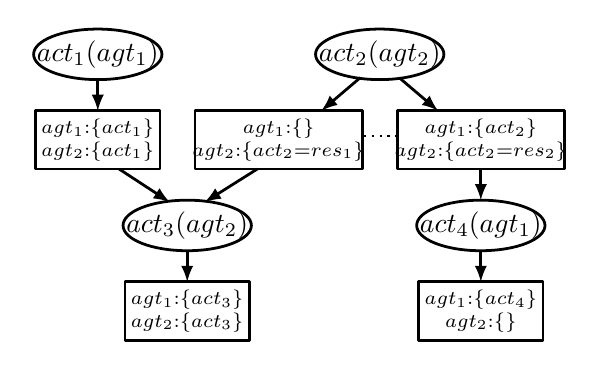
\begin{tikzpicture}[>=latex,join=bevel,scale=0.7]
  \pgfsetlinewidth{1bp}
%
\pgfsetcolor{black}
  % Edge: n1 -> n2
  \draw [->] (33bp,194bp) -- (33bp,178bp);
  % Edge: n3 -> n4
  \draw [->] (168bp,195bp) -- (148bp,178bp);
  % Edge: n3 -> n5
  \draw [->] (188bp,195bp) -- (208bp,178bp);
  % Dotted Edge n4 -- n5
  \draw [-,dotted,thick] (170bp,165bp) -- (188bp,165bp);
  % Edge: n6 -> n7
  \draw [->] (79bp,106bp) -- (79bp,90bp);
  % Edge: n8 -> n9
  \draw [->] (230bp,106bp) -- (230bp,90bp);
  % Edge: n2 -> n6
  \draw [->] (44bp,148bp) -- (70bp,131bp);
  % Edge: n4 -> n6
  \draw [->] (115bp,148bp) -- (88bp,131bp);
  % Edge: n5 -> n8
  \draw [->] (230bp,148bp) -- (230bp,132bp);
  % Node: n1
\begin{scope}
  \pgfsetstrokecolor{black}
  \draw (33bp,207bp) ellipse (33bp and 13bp);
  \draw (33bp,207bp) node {$act_1(agt_1)$};
\end{scope}
  % Node: n2
\begin{scope}
  \pgfsetstrokecolor{black}
  \draw (65bp,178bp) -- (1bp,178bp) -- (1bp,148bp) -- (65bp,148bp) -- cycle;
  \draw (33bp,163bp) node {$agt_1: \{act_1\} \atop agt_2: \{act_1\}$};
\end{scope}
  % Node: n3
\begin{scope}
  \pgfsetstrokecolor{black}
  \draw (178bp,207bp) ellipse (33bp and 13bp);
  \draw (178bp,207bp) node {$act_2(agt_2)$};
\end{scope}
  % Node: n4
\begin{scope}
  \pgfsetstrokecolor{black}
  \draw (169bp,178bp) -- (83bp,178bp) -- (83bp,148bp) -- (169bp,148bp) -- cycle;
  \draw (126bp,163bp) node {$agt_1: \{\} \atop agt_2: \{act_2=res_1\}$};
\end{scope}
  % Node: n5
\begin{scope}
  \pgfsetstrokecolor{black}
  \draw (273bp,178bp) -- (187bp,178bp) -- (187bp,148bp) -- (273bp,148bp) -- cycle;
  \draw (230bp,163bp) node {$agt_1: \{act_2\} \atop agt_2: \{act_2=res_2\}$};
\end{scope}
  % Node: n6
\begin{scope}
  \pgfsetstrokecolor{black}
  \draw (79bp,119bp) ellipse (33bp and 13bp);
  \draw (79bp,119bp) node {$act_3(agt_2)$};
\end{scope}
  % Node: n7
\begin{scope}
  \pgfsetstrokecolor{black}
  \draw (111bp,90bp) -- (47bp,90bp) -- (47bp,60bp) -- (111bp,60bp) -- cycle;
  \draw (79bp,75bp) node {$agt_1: \{act_3\} \atop agt_2: \{act_3\}$};
\end{scope}
  % Node: n8
\begin{scope}
  \pgfsetstrokecolor{black}
  \draw (230bp,119bp) ellipse (33bp and 13bp);
  \draw (230bp,119bp) node {$act_4(agt_1)$};
\end{scope}
  % Node: n9
\begin{scope}
  \pgfsetstrokecolor{black}
  \draw (262bp,90bp) -- (198bp,90bp) -- (198bp,60bp) -- (262bp,60bp) -- cycle;
  \draw (230bp,75bp) node {$agt_1: \{act_4\} \atop agt_2: \{\}$};
\end{scope}
%
\end{tikzpicture}

